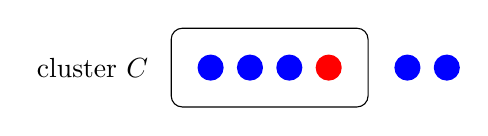
\begin{tikzpicture}
            [   cnode/.style={fill=blue, circle},
            ]
            \def\x{0.5};
            \def\recx{-0.5};
            \node [cnode] at (0, 0) {};
            \node [cnode] at (1*\x, 0) {};
            \node [cnode] at (2*\x, 0) {};
            \node [fill=red, circle] at (3*\x, 0) {};
            \node [cnode] at (5*\x, 0) {};
            \node [cnode] at (6*\x, 0) {};
            \draw[rounded corners] (-\x, -\x) rectangle (4*\x, \x) {};
            \node [] at (-1.5, 0) {cluster $C$};  
        \end{tikzpicture}